\begingroup\emergencystretch=3em
\section{Eksplorasi Data}
\label{sec:eda}

Eksplorasi data (\textit{exploratory data analysis}, EDA) dilakukan pada data latih di \texttt{src/kaggle/eda.ipynb}, dan seluruh gambar tersimpan di \texttt{output/eda/}. Tujuannya memahami struktur, kualitas, dan pola data sebelum algoritma dibangun, sehingga keputusan \textit{cleaning} dan \textit{preprocessing} pada tiap algoritma didukung bukti. Data latih dan data uji tidak pernah digabung; data uji hanya dipakai untuk membandingkan distribusi dan kualitasnya.

\subsection{Kualitas Data}
\label{subsec:kualitas-data}

\paragraph{Nilai hilang.} Delapan kolom memiliki nilai kosong sebesar 2,96\% sampai 11,09\% (Gambar~\ref{fig:missing-pct}), dengan pola yang hampir sama pada data uji. Hanya 60,8\% baris yang lengkap: 8.478 baris kehilangan satu kolom, 1.933 baris dua kolom, dan sisanya tiga sampai lima kolom. Menghapus baris yang tidak lengkap akan membuang 39,2\% data, dan cara itu tidak dapat diterapkan pada data uji karena semua barisnya harus diprediksi. Imputasi karena itu wajib.

Hubungan kekosongan dengan target diuji dengan uji \textit{chi-square} antara indikator ``kosong'' dan target, dengan koreksi Bonferroni. Hanya \texttt{special\_\allowbreak requests} yang kekosongannya berkaitan dengan target: tingkat batal 40,8\% saat kosong dan 31,9\% saat terisi. Tujuh kolom lain tidak signifikan, sehingga imputasi sederhana memadai untuk kolom tersebut. Kekosongan \texttt{special\_\allowbreak requests} condong ke nilai nol: pada kanal \textit{Online Travel Agent}, tingkat batal baris kosong menyiratkan sekitar 83\% di antaranya bernilai nol, padahal hanya 36,6\% baris terisi yang bernilai nol. Imputasi dengan median (yaitu 0) sesuai dengan nilai yang paling mungkin, dan indikator kosong dapat ditambahkan sebagai fitur.

\begin{figure}[H]
	\centering
	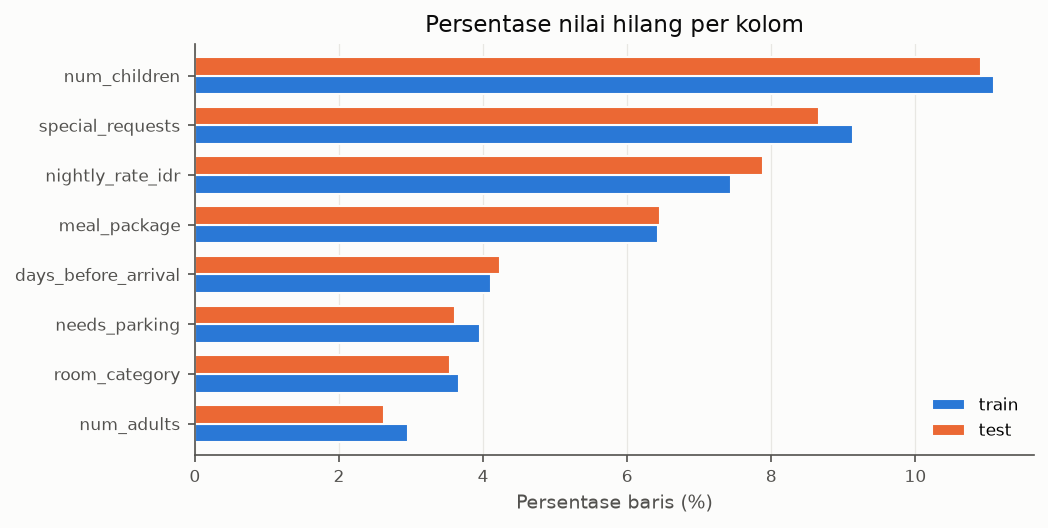
\includegraphics[width=0.75\textwidth]{missing_pct.png}
	\caption{Persentase nilai hilang per fitur pada data latih dan data uji}
	\label{fig:missing-pct}
\end{figure}

\paragraph{Duplikat.} Kolom \texttt{id} selalu unik, sehingga duplikat diperiksa pada seluruh fitur. Terdapat 62 grup duplikat dengan 66 baris berlebih, dan 2 grup memiliki label yang berbeda. Membuang duplikat identik beserta labelnya menghapus 64 baris (0,2\%), sehingga dampaknya kecil. Selain itu, 42 baris data uji memiliki fitur yang sama dengan baris data latih. Baris uji tersebut tetap harus diprediksi dan tidak boleh dihapus.

\paragraph{Nilai tidak wajar.} Beberapa kombinasi nilai tampak tidak masuk akal, tetapi ternyata informatif dan juga muncul pada data uji, sehingga tidak dihapus (Tabel~\ref{tab:anomali}). Sebagai contoh, \texttt{num\_adults} $=0$ bukan kesalahan data, karena 105 dari 106 baris memiliki anak dan satu sisanya kosong. Tarif nol hampir selalu tidak batal (0,7\%); dari 413 barisnya, 267 berasal dari kanal \textit{Complimentary} (tidak pernah batal) dan 146 dari \textit{Online Travel Agent} (2,1\% batal). Median tarif kanal \textit{Complimentary} adalah 0 sedangkan median keseluruhan 1,644 juta, sehingga imputasi tarif dengan median global akan keliru pada kanal ini dan imputasi per kanal lebih tepat. Kolom \texttt{is\_\allowbreak returning\_\allowbreak guest} juga sepenuhnya konsisten dengan riwayat pesanan sebelumnya. Hanya \texttt{num\_children} $\ge 9$ dan tarif di atas 6 juta yang layak dipangkas, masing-masing 3 baris dan tidak ada pada data uji.

\begin{table}[H]
	\centering
	\caption{Nilai tidak wajar pada data latih dan data uji}
	\label{tab:anomali}
	\begin{tabular}{l r c r}
		\toprule
		\textbf{Aturan} & \textbf{Baris latih} & \textbf{Tingkat batal} & \textbf{Baris uji} \\
		\midrule
		\texttt{num\_adults} $= 0$ & 106 & 0,302 & 22 \\
		total malam $= 0$ & 64 & 0,031 & 9 \\
		\texttt{nightly\_\allowbreak rate\_\allowbreak idr} $= 0$ & 413 & 0,007 & 85 \\
		\texttt{num\_children} $\ge 9$ & 3 & 0,333 & 0 \\
		\texttt{prior\_\allowbreak cancellations} $\ge 10$ & 21 & 0,095 & 8 \\
		total malam $\ge 15$ & 55 & 0,800 & 12 \\
		tarif $> 6$ juta & 3 & 0,667 & 0 \\
		\bottomrule
	\end{tabular}
\end{table}

\subsection{Distribusi Fitur Numerik}
\label{subsec:eda-numerik}

\paragraph{Fitur kontinu.} \texttt{days\_\allowbreak before\_\allowbreak arrival} adalah fitur terkuat. Tingkat batal naik dari 8,5\% pada desil terendah (0 sampai 4 hari) ke 75,7\% pada desil tertinggi (di atas 213 hari), dengan lompatan tajam dari 36,3\% ke 68,0\% di sekitar 151 hari. Hubungan ini monotonik tetapi tidak linear. Sebaliknya, \texttt{nightly\_\allowbreak rate\_\allowbreak idr} tidak monotonik: tingkat batal naik sampai puncak 47,5\% pada tarif sekitar 1,8 sampai 1,9 juta, lalu turun lagi, sedangkan tarif nol membentuk kelompok tersendiri yang hampir tidak pernah batal. Model linear tidak dapat menangkap bentuk ini tanpa transformasi fitur.

\begin{figure}[H]
	\centering
	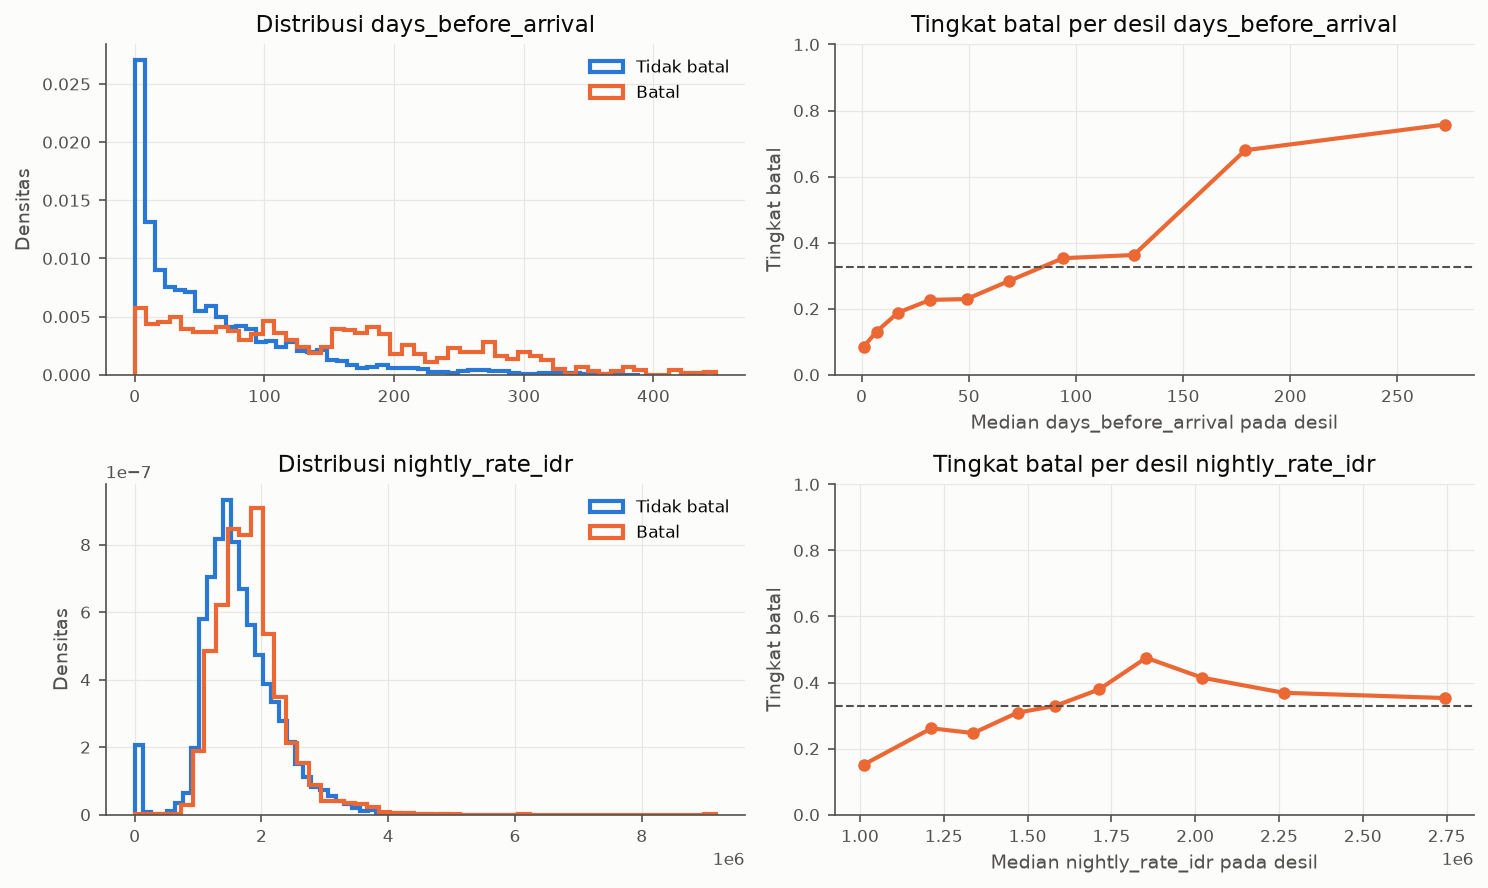
\includegraphics[width=0.9\textwidth]{continuous_features.png}
	\caption{Distribusi fitur kontinu menurut kelas target (kiri) dan tingkat batal per desil (kanan)}
	\label{fig:continuous-features}
\end{figure}

\paragraph{Fitur hitungan dan biner.} \texttt{special\_\allowbreak requests} adalah sinyal negatif terkuat: tingkat batal turun dari 43,2\% pada nilai 0 ke 23,8\% dan 14,3\% pada nilai 1 dan 2, lalu 0\% untuk seluruh 563 baris dengan nilai minimal 3. Tamu lama (1,5\% batal), kebutuhan parkir (10,1\%), dan riwayat pembatalan cenderung menurunkan risiko, sedangkan masa inap panjang cenderung menaikkannya. \texttt{num\_adults} dan \texttt{num\_children} lemah.

\subsection{Distribusi Fitur Kategorikal}
\label{subsec:eda-kategorikal}

Ketiga fitur kategorikal berhubungan signifikan dengan target menurut uji \textit{chi-square} ($p < 10^{-7}$), tetapi kekuatannya berbeda (Gambar~\ref{fig:categorical-rates}). \texttt{booking\_\allowbreak channel} paling kuat: kanal \textit{Complimentary} tidak pernah batal, \textit{Corporate} 11,5\%, dan \textit{Online Travel Agent} 36,4\%. Pada \texttt{meal\_package}, \textit{Half Board} menonjol dengan 45,9\%. \texttt{room\_\allowbreak category} paling lemah. Beberapa kategori sangat langka: \textit{Full Board} hanya 4 baris dan Type E hanya 7 baris pada data latih (tidak ada Type E pada data uji), sehingga \textit{one-hot encoding} akan menghasilkan kolom yang hampir selalu nol dan kategori langka perlu digabung. Baris kosong pada kedua kolom itu memiliki tingkat batal mendekati rata-rata, sehingga cukup diberi kategori sendiri. Tidak ada kategori baru pada data uji.

\begin{figure}[H]
	\centering
	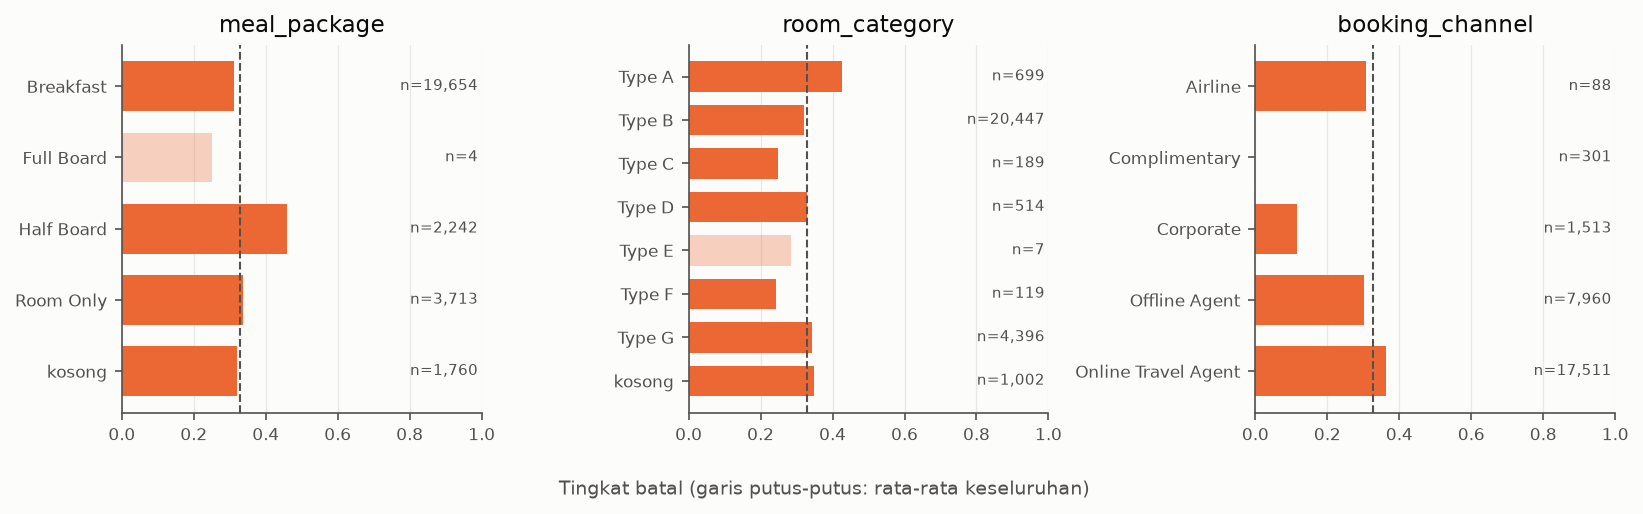
\includegraphics[width=\textwidth]{categorical_rates.png}
	\caption{Tingkat pembatalan per kategori (garis putus-putus: rata-rata keseluruhan; $n$ pada tiap batang)}
	\label{fig:categorical-rates}
\end{figure}

\subsection{Pola Waktu}
\label{subsec:eda-waktu}

Data latih dan data uji mencakup rentang tanggal kedatangan yang sama (1 Juli 2023 sampai 30 Desember 2024), dan porsi data uji per bulan stabil pada 19,0\% sampai 22,8\%. Artinya pembagian data bersifat acak, bukan berdasarkan waktu, sehingga \textit{stratified k-fold} mewakili kondisi data uji pada Kaggle.

Periode kedatangan membawa sinyal yang besar (Gambar~\ref{fig:monthly-trend}). Tingkat batal bergerak dari 2,5\% pada Desember 2023 hingga 64,2\% pada Juli 2023, walaupun Juli 2023 hanya memuat 274 baris. Pola ini bukan musiman murni: Oktober bernilai 16,2\% pada 2023 dan 46,5\% pada 2024, sedangkan Juli bernilai 64,2\% dan 42,0\%. Karena itu \texttt{arrival\_\allowbreak month} saja tidak cukup, dan kombinasi tahun dan bulan lebih informatif. Hari kedatangan (30,5\% sampai 37,2\%) dan tanggal (26,8\% sampai 40,7\%) jauh lebih lemah. Efek \textit{lead time} juga bergantung pada periode: \textit{lead time} 151 sampai 250 hari memiliki tingkat batal 0,72 sampai 0,82 pada Mei hingga Oktober 2024, tetapi hanya 0,38 pada Desember 2024.

Bulan pemesanan dapat diturunkan dari tanggal kedatangan dikurangi \texttt{days\_\allowbreak before\_\allowbreak arrival}. Fitur ini diketahui saat pesanan dibuat, sehingga tidak membocorkan target, dan memiliki sinyal yang tidak identik dengan bulan kedatangan (misalnya lompatan dari 17,3\% pada September 2023 ke 45,1\% pada Oktober 2023). Penurunan hingga 0,3\% pada Desember 2024 perlu dibaca hati-hati: seluruh kedatangan berakhir pada Desember 2024, sehingga pesanan pada bulan itu pasti berlead time pendek, yang memang jarang batal.

Satu catatan penting: fitur periode efektif untuk Kaggle karena data uji berada pada periode yang sama dengan data latih, tetapi tidak akan berlaku untuk bulan yang belum pernah terlihat pada penerapan nyata.

\begin{figure}[H]
	\centering
	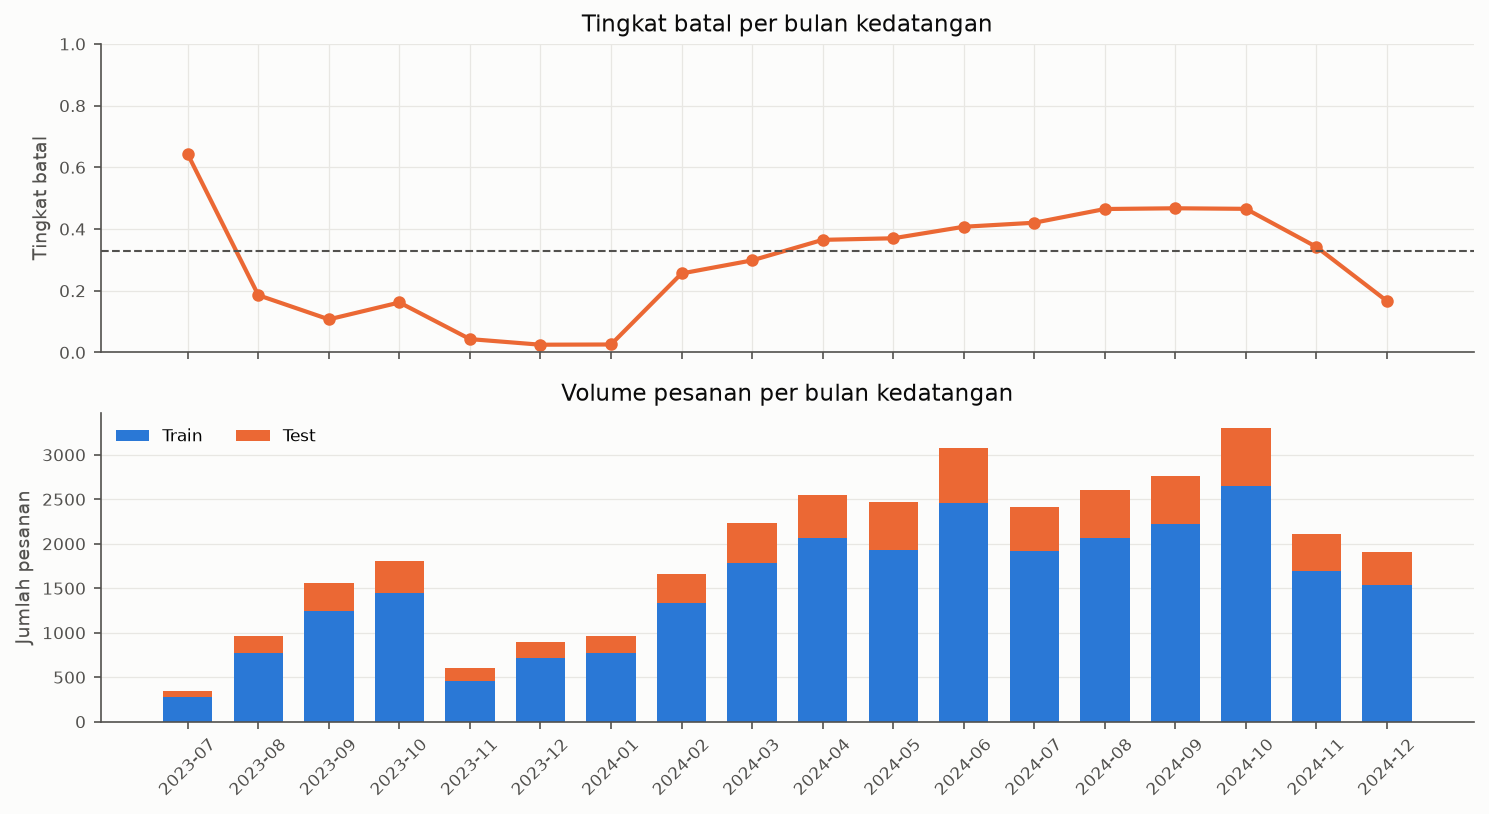
\includegraphics[width=0.9\textwidth]{monthly_trend.png}
	\caption{Tingkat pembatalan (atas) dan volume pesanan (bawah) per bulan kedatangan}
	\label{fig:monthly-trend}
\end{figure}

\subsection{Korelasi dan Relevansi Fitur}
\label{subsec:eda-korelasi}

Korelasi Spearman dipilih karena banyak fitur miring dan berupa hitungan. Korelasi terhadap target terkuat dimiliki \texttt{days\_\allowbreak before\_\allowbreak arrival} (0,418) dan \texttt{special\_\allowbreak requests} ($-0{,}261$), disusul \texttt{arrival\_year} (0,180) dan \texttt{nightly\_\allowbreak rate\_\allowbreak idr} (0,148). Redundansi utama hanya satu kelompok, yaitu riwayat tamu: \texttt{prior\_\allowbreak completed\_\allowbreak bookings} dengan \texttt{is\_\allowbreak returning\_\allowbreak guest} (0,932) dan \texttt{prior\_\allowbreak cancellations} dengan \texttt{is\_\allowbreak returning\_\allowbreak guest} (0,587). Pasangan fitur lain tidak berkorelasi tinggi.

Korelasi hanya menangkap hubungan monotonik, sehingga \textit{mutual information} (MI) ikut dihitung pada data latih setelah imputasi sementara, dan Cram\'er's V untuk fitur kategorikal. MI menempatkan \texttt{days\_\allowbreak before\_\allowbreak arrival} di puncak (0,105), diikuti \texttt{arrival\_ym}, yaitu kombinasi tahun dan bulan kedatangan (0,052), \texttt{special\_\allowbreak requests} (0,037), dan bulan pemesanan (0,028). \texttt{arrival\_ym} jauh melampaui \texttt{arrival\_\allowbreak month} (0,025) dan memiliki Cram\'er's V tertinggi (0,298), yang mendukung penggunaan kombinasi tahun-bulan. \texttt{room\_\allowbreak category} dan \texttt{num\_children} memiliki MI terendah. Ukuran ini univariat dan tidak melihat interaksi, sehingga fitur yang lemah tidak langsung dibuang; pemilihan fitur diputuskan melalui validasi silang pada tiap algoritma.

\begin{figure}[H]
	\centering
	\begin{subfigure}{0.48\textwidth}
		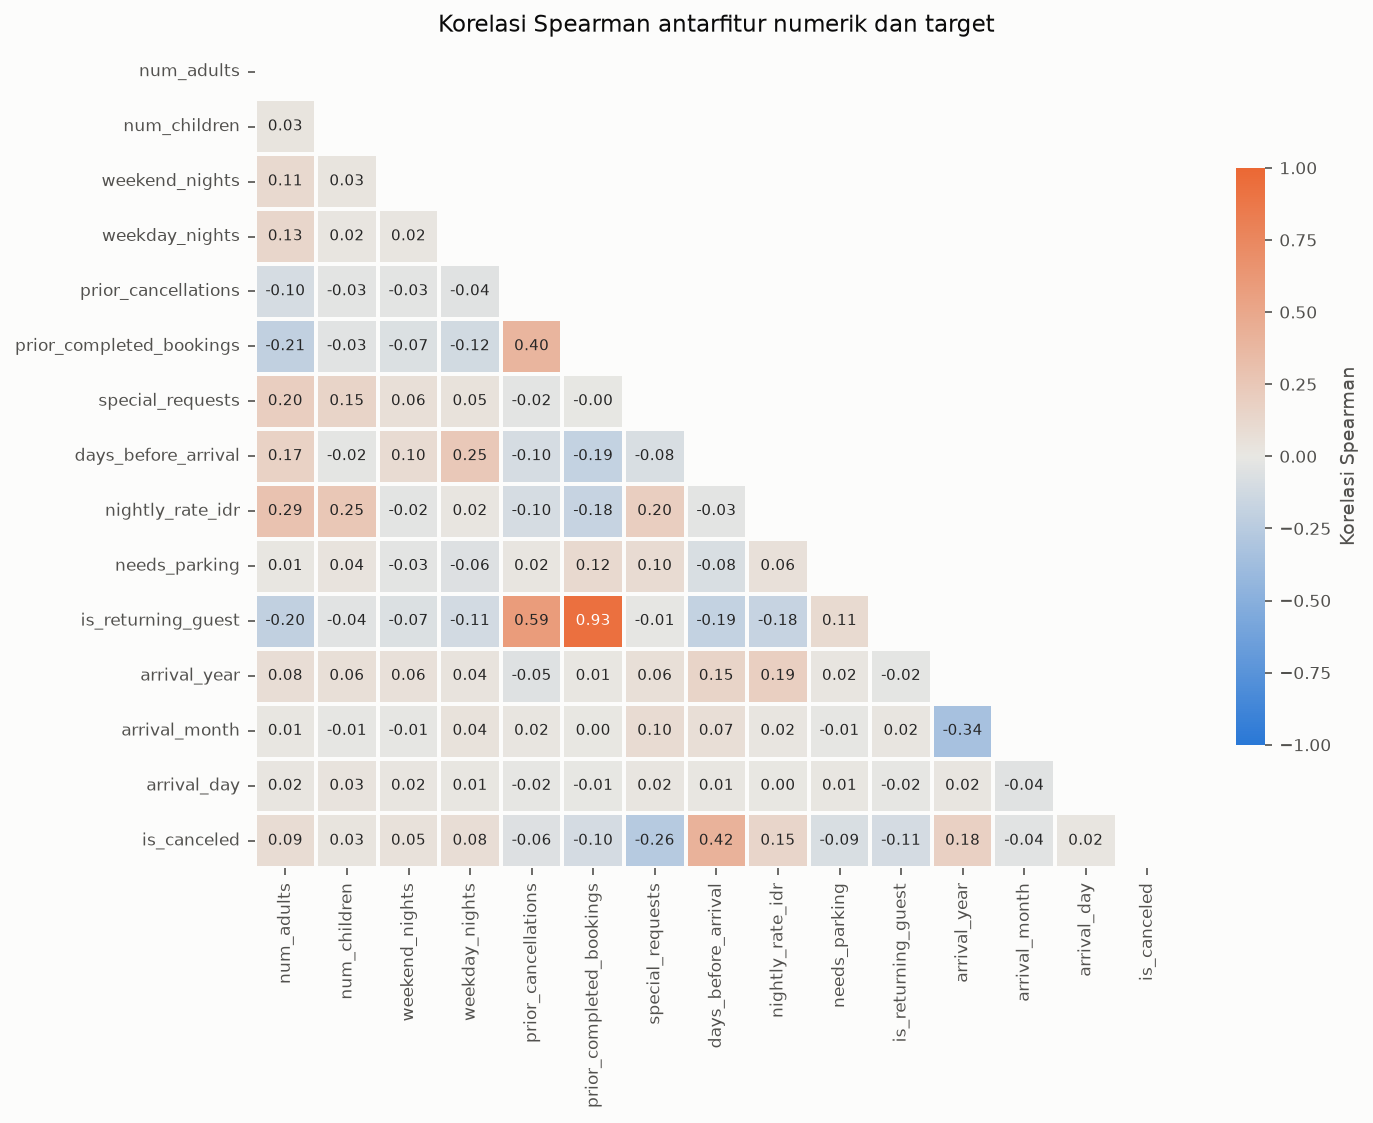
\includegraphics[width=\textwidth]{spearman_correlation.png}
		\caption{Korelasi Spearman}
	\end{subfigure}
	\hfill
	\begin{subfigure}{0.48\textwidth}
		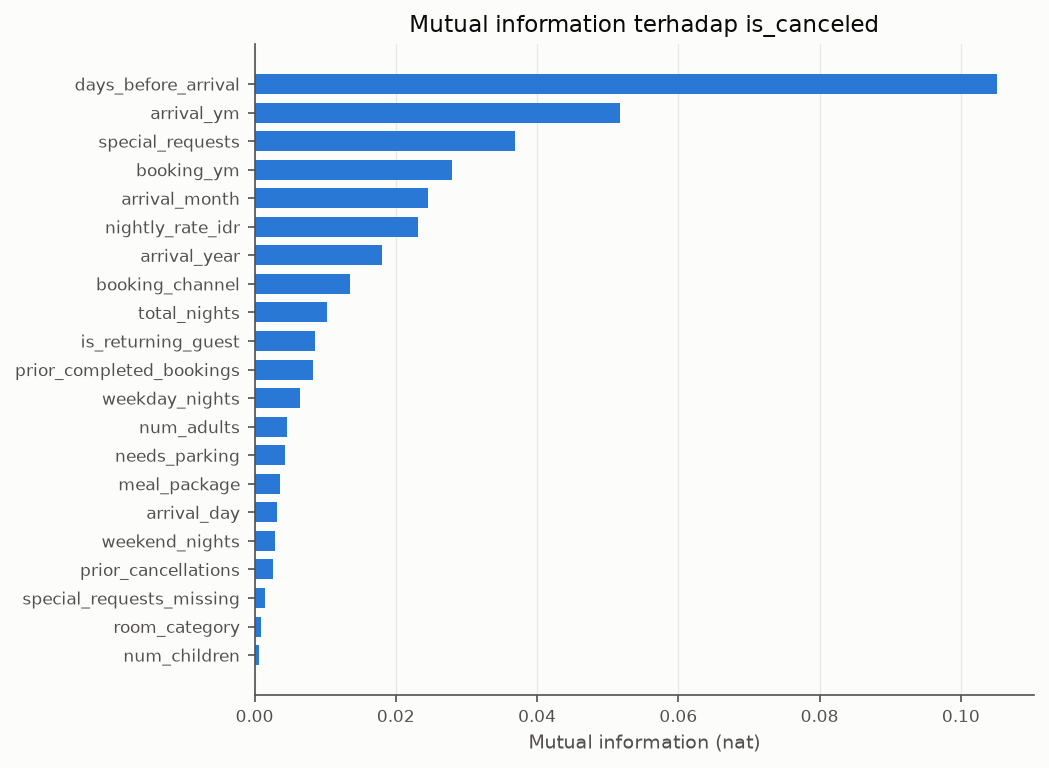
\includegraphics[width=\textwidth]{mutual_information.png}
		\caption{\textit{Mutual information}}
	\end{subfigure}
	\caption{Relevansi fitur terhadap target}
	\label{fig:relevansi-fitur}
\end{figure}

\subsection{Perbandingan Data Latih dan Data Uji}
\label{subsec:eda-train-test}

Skor validasi hanya mewakili skor data uji jika kedua berkas berasal dari distribusi yang sama. Pergeseran distribusi diukur dengan \textit{Population Stability Index} (PSI), dengan batas (\textit{bin}) dari data latih dan data uji dievaluasi pada batas tersebut sehingga kedua berkas tetap terpisah, serta statistik Kolmogorov-Smirnov (KS) untuk fitur numerik. PSI tertinggi hanya 0,0021 dan KS tertinggi 0,0149, jauh di bawah batas kestabilan 0,1, dan tidak ada kategori baru pada data uji. Tidak ada pergeseran distribusi, sehingga skor validasi silang dapat dijadikan perkiraan skor data uji.

\subsection{Ringkasan Temuan}
\label{subsec:ringkasan-eda}

EDA ini adalah tahap \textit{data understanding} pada kerangka CRISP-DM \cite{slide-crispdm}: memahami struktur, kualitas, dan pola data sebelum \textit{data preparation} dan pemodelan. Temuan utama dan keputusan yang diturunkannya dirangkum pada Tabel~\ref{tab:ringkasan-eda}, dan menjadi dasar subbab \textit{preprocessing} tiap algoritma di Bab~2. Kolom kanan adalah implikasi yang disarankan EDA; keputusan akhir tiap algoritma dibahas pada subbabnya masing-masing dan dapat berbeda karena kebutuhan algoritmanya.

\begin{table}[H]
	\centering
	\caption{Temuan EDA dan implikasinya untuk \textit{preprocessing}}
	\label{tab:ringkasan-eda}
	\begin{tabular}{p{6.4cm} p{6.4cm}}
		\toprule
		\textbf{Temuan} & \textbf{Implikasi untuk \textit{preprocessing}} \\
		\midrule
		Hanya 60,8\% baris lengkap; delapan kolom memiliki nilai hilang & Imputasi (median untuk numerik, kategori sendiri untuk kategorikal), bukan hapus baris \\
		Kekosongan \texttt{special\_\allowbreak requests} berkaitan dengan target & Tambahkan indikator kosong \\
		Tarif nol hampir semuanya kanal \textit{Complimentary}; median tarif per kanal berbeda & Imputasi tarif per kanal lebih tepat daripada median global \\
		64 baris duplikat identik (0,2\%) & Buang duplikat pada data latih saja, data uji tidak disentuh \\
		Nilai ekstrem informatif dan muncul juga pada data uji & Tidak dihapus; pangkas hanya tiga baris ekstrem \\
		\texttt{days\_\allowbreak before\_\allowbreak arrival} dan \texttt{nightly\_\allowbreak rate\_\allowbreak idr} berhubungan nonlinear dengan target & Transformasi (misalnya logaritma) dan fitur interaksi untuk model linear \\
		Kategori sangat langka (\textit{Full Board}, Type E) & Gabungkan kategori langka sebelum \textit{one-hot} \\
		Periode kedatangan dan pemesanan membawa sinyal besar, dan data uji berada pada periode yang sama & Pakai kombinasi tahun-bulan sebagai fitur; hanya sah untuk Kaggle, bukan untuk periode baru \\
		\texttt{prior\_\allowbreak completed\_\allowbreak bookings} berkorelasi 0,932 dengan \texttt{is\_\allowbreak returning\_\allowbreak guest} & Redundan, dipertimbangkan pada \textit{feature selection} \\
		Skala fitur sangat timpang & Standardisasi, di-\textit{fit} hanya pada data latih \\
		Kelas tidak seimbang moderat (2,05 : 1) & \textit{Threshold} dipilih untuk Macro F1, tanpa \textit{resampling} \\
		Tidak ada pergeseran distribusi (PSI $< 0{,}003$) & Validasi silang mewakili skor data uji \\
		\bottomrule
	\end{tabular}
\end{table}
\endgroup
